\documentclass[preprint2]{aastex}
\usepackage[colorlinks]{hyperref}
\usepackage{amsmath, bm}
\usepackage{fancyhdr}
\usepackage{floatrow}
\usepackage[inner=2cm,outer=2cm,bottom=1cm,top=1.5cm]{geometry}
%\usepackage{mathtools}
\usepackage{multicol}
\usepackage{verbatim}
\usepackage{graphicx,float,wrapfig, subcaption}
\usepackage{indentfirst}
\usepackage{soul}

\fancyhf{} % clear all header and footers
\renewcommand{\headrulewidth}{0pt} % remove the header rule
\rhead{\thepage}

%
%lfoot{\thepage} % puts it on the left side instead
%
% or if your document is 2 sided, and you want even and odd placement of the number
%facncyfoot[LE,RO]{\thepage} % Left side on Even pages; Right side on Odd pages
%
\pagestyle{fancy}

\begin{document}

\title{Differentially Private Interactive Media}

\author{\vspace{-0.5cm}{\hspace{0.1cm} \sc Jan Van Bruggen \hspace{1.6cm} James Chang \hspace{1.6cm} Cutter Coryell}} \email{jvanbrug@caltech.edu \hspace{1.3cm} jcchang@caltech.edu \hspace{1.1cm} ccoryell@caltech.edu}
\vspace{0.2cm}\affil{California Institute of Technology \vspace{1cm}}



\section{Introduction}

In the modern era, entities who own and sell digital content are increasingly concerned with unauthorized access to that content. A variety of ``digital rights management'' (DRM) technologies have been introduced to attempt to restrict content access to authorized users, with mixed results. In many cases arms races have resulted between content-providers and users in terms of rights management technologies and methods for breaking them. These technologies usually make it hard to share content between authorized users and unauthorized users and are commonly criticized for inconveniencing authorized users --- some content-providers push their lack of DRM as a selling point, and a general anti-DRM movement has sprung up.

One way to prevent unauthorized sharing of content is to change the nature of the content to make it fundamentally unsharable. For example, by \emph{streaming} content as opposed to handing out content in bundles which can be saved locally, it becomes non-trivial for the regular user to share their received content. Many music, movie/television, and even video-game services take this approach to control content access. However, it is not difficult for an unauthorized user to record the data stream in a way that can be saved locally, such that he manufactures his own content bundles which he can share. We say that the user has \emph{fully reconstructed} the content if she can provide an identical experience to an unauthorized user as an authorized user would receive through the official content channel.

It becomes significantly harder for a user to fully reconstruct the original content if the streamed content is in some way interactive. For example, in a streamed video-game, the data that is streamed to the user depends on the the input that the user provides. In order to provide the same experience to unauthorized users as the one that authorized users receive, the reconstructor must provide every possible time series of inputs to the content provider and record every resulting stream. If the content is deterministic --- the same time series of inputs always leads to the same data stream --- then this reconstruction ensures that any inputs that authorized users can give can also be given by unauthorized users \emph{with the same results}. This satisfies our definition of full reconstruction, because the experience of the unauthorized user is identical to that of the authorized user.\footnote{We define two users to have\emph{ identical experience} if, given the same time series of user inputs, the true probability distributions of certain content being streamed to each user is the same. This will be further motivated when we discuss noise in streaming.}

Yet another change that can be made to how content is provided to make reconstruction more difficult is the addition of noise. This method is motivated by differential privacy, which is a notion of how the probability of a certain output to a query will change given a change in the queried database. By adding noise to a query in a special way, the particular existence or absence of a datum in the database can be concealed while still revealing useful information that respects differential privacy. The general idea of using noise to make it harder to reconstruct content is one we would like to borrow. With noise,\footnote{To be clear, when we refer to \emph{noise} we mean simply the introduction of randomness in the potential stream output --- far more general than the literal addition of noise values to the data.} every stream a content provider serves to a user is a random variable. Someone attempting to reconstruct the original content who, as before, only samples from the stream once (or once for every possible input time series if the content is interactive) will provide users with an empirical probability distribution where only one output has nonzero probability: that particular output the reconstructor sampled from the original content provider. This is quite possibly a poor approximation to the actual probability distribution governing possible outputs in the official stream.

How interactivity and noise make reconstruction harder, both individually and together, is an interesting question that we attempt to answer.

\section{Methods}

To investigate how the ease of reconstruction of a specific content-base depends on the interactiveness of the content stream and on the noise added to the content stream, we set up two simple models. In the first model, which lacks interaction, there is a space of possible outputs with utilities assigned by the content-creator --- the particular output given to a user is chosen by the \emph{exponential mechanism} from the differential privacy literature.

The output for the second model is a Markovian sequence of items. The probability of any particular item appear at a certain position in the sequence is determined entirely from the previous item in the sequence. The first item of the sequence is chosen uniformly randomly, and subsequent items are chosen via the exponential mechanism. As in the first model, the content-creator assigns utilities to each item-to-item transition which are used by the exponential mechanism. However, in this model we allow for interaction. At query-time, the user provides a vector of preferences, one for each item in the item space. The utilities of the transitions away from a particular item are allowed to be functions of the user preference value for that item.

We now develop the two models mathematically.

\subsection{Model 1}

Let \(\mathcal{S}\) be the set of all possible outputs to a streaming query. Let \(\mathcal{I} \subseteq \mathcal{S}\) be a set of \emph{intended} outputs --- these being, informally, the outputs that the content-creator actually wishes the users to receive in the absence of noise. The content creator specifies \(\mathbf{u} = [(u_1, s_1), (u_2, s_2), (u_3, s_3), \dots]\), where each \(u_j \in (0, 1]\) is a utility and each \(s_j \in \mathcal{S}\). Here, \(\mathbf{u}\) is a multiset (elements can occur more than once) with any desired cardinality. In terms of differential privacy, \(\mathbf{u}\) is a database. We have \(\mathcal{I} = \mathcal{I}(\mathbf{u}) \equiv \{s \in \mathcal{S} \ | \ \exists \ u \text{ s.t. } (u, s) \in \mathbf{u}\}\).

The sampling mechanism is defined as follows: \\

\noindent\(sample_1(\mathbf{u}, \varepsilon):\) \\
\indent Output \(s \in \mathcal{S}\) with probability \(\propto \exp \left( \frac{1}{2} \varepsilon U(s) \right)\) \\

\noindent where \(U(s) \equiv u_j\) if \(s = s_j \in \mathcal{I}\) or \(U(s) = 0\) if \(s \notin \mathcal{I}\).

This mechanism is the exponential mechanism of differential privacy with privacy parameter \(\varepsilon\) where the utility function is defined over the outcome space of all possible outputs, including unintended outputs. The sensitivity of \(U(s)\) is 1 because \(U(s) \in [0, 1]\) and is implicitly in the mechanism definition. Because it is just an application of the exponential mechanism, \(sample_1\) is \(\varepsilon\)-differentially private. What this means intuitively is that the change in probability of a certain output being sampled if the output (or any other output, in fact) changes from intended to unintended (or back) cannot be more than a certain factor --- \(e^\varepsilon\) to be precise.

The interesting question to be answered by this model is how the reconstruction quality of \(\mathbf{u}\) changes with \(\varepsilon\) and with the number of queries to \(sample_1(\mathbf{u}, \varepsilon)\). What the reconstructor, which we shall refer to as the adversary henceforth, tries to build is a probability distribution over \(\mathcal{S}\), \(p_\text{approx}(s)\) which approximates the true probability distribution \(p(s)\) over outputs of \(sample_1(\mathbf{u}, \varepsilon)\). There are many conceivable ways to generate \(p_\text{approx}(s)\) from a finite number of samples --- the most straightforward of which is constructing an empirical distribution where the probability of \(s\) is equal to the proportion of all outputs that were \(s\). There are also many conceivable ways to measure the quality of \(p_\text{approx}(s)\) in approximating \(p(s)\), but a common one and the one we choose to use here is the KL-divergence, defined as follows:
\[
\text{div}_{KL}(p||p_\text{approx}) \equiv \sum_{s \in \mathcal{S}} p(s) \log \frac{p(s)}{p_\text{approx}(s)}
\]

By inspection, the KL-divergence is not defined unless \(p_\text{approx}(s) = 0 \Rightarrow p(s) = 0\). It is clear that the KL-divergence is not defined for the empirical distribution until every possible sequence has been sampled at least once, which may take a very large number of samples. Therefore we use an alternate method for generating \(p_\text{approx}(s)\) that is compatible with our choice of the KL-divergence for comparing \(p_\text{approx}(s)\) to \(p(s)\) --- Multiplicative Weights. This algorithm is given below: \\

\noindent \(MW_1(N, \eta):\)\\
\indent Set \(w_s \leftarrow 1 \ \forall \ s \in \mathcal{S}\) \\
\indent Repeat \(N\) times:\\
\indent \indent Sample \(\sigma \leftarrow sample_1(\mathbf{u}, \varepsilon)\) \\
\indent \indent Set \(w_\sigma \leftarrow w_\sigma e^\eta\) \\
\indent Output \(p_\text{approx}(s) \propto w_s \) \\

In words, Multiplicative Weights initially assigns equal probability to all possible outputs, then samples from the mechanism \(N\) times, increasing the probabilities of outputs that occur at the expense of the probabilities of all other outputs. In order to do this, the update parameter \(\eta\) must be given, which controls how much the probability of each output changes when the output occurs. It is clear that \(MW_1\) will always output an approximate probability distribution that leads to a defined KL-divergence for any true probability distribution.

\subsection{Model 2}

Let \(\mathcal{C}\) be the content universe. The set of all possible outputs is \(\mathcal{S} \equiv \mathcal{C}^n\) --- that is, an output is a sequence \(s = (c_1, c_2, \dots, c_n)\) for \(c_j \in \mathcal{C}\) and for some sequence length \(n\). Define a graphical network \(\mathcal{N} \equiv (\mathcal{C}, \mathcal{E})\) where \(\mathcal{E}\) is a multiset of directed edges with edge weights between nodes in \(\mathcal{C}\). Specifically, an edge is of the form \(\epsilon = (c_\text{source}, c_\text{destination}, \rho, u)\), where the source node \(c_\text{source}\) and the destination node \(c_\text{destination}\) are both in \(\mathcal{C}\), \(\rho \in \mathcal{P}\) is a particular possible value for a preference that the user is allowed to choose at query-time defined by the content-creator, and \(u \in (0, 1]\) is a utility defined by the content-creator. \(\mathcal{P}\) is the set of possible preferences at each node, which is assumed to be constant over the nodes for now --- this can be interpreted as a set of options presented to the user when he arrives at a node. Here, \(\mathcal{E}\) can be considered the private database, as \(\mathcal{C}\) is assumed public knowledge. The content-creator is free to define as many or as few edges as she wishes.

The sampling mechanism is defined as follows: \\
\newpage
\noindent\(sample_2(\mathcal{N}, P, n, \varepsilon):\) \\
\indent Set \(c_1 \leftarrow c \in \mathcal{C}\) with probability \(1 / |\mathcal{C}|\) \\
\indent For \(i = 2, \dots, n\):\\
\indent \indent Set \(c_i \leftarrow c \in \mathcal{C}\) with probability \(\propto \exp\left( \frac{1}{2} \varepsilon U(c | c_{i-1}) \right)\)
\indent Output \(s = (c_1, c_2, \dots, c_n)\) \\

In this mechanism, \(\mathcal{N} = (\mathcal{C}, \mathcal{E})\) is the content network, \(P : \mathcal{C} \rightarrow \mathcal{P}\) is a mapping between content nodes and a user-given preference for each node, \(n\) is the sequence length, \(\varepsilon\) is the privacy parameter, and \(s\) is the output sequence. The utility function \(U(c|c') = u \Leftrightarrow (c', c, P(c'), u) \in \mathcal{E}\), and \(U(c|c') = 0 \Leftrightarrow (c', c, P(c'), u) \notin \mathcal{E} \ \forall\  u\). In words, if there is an edge defined in the content network that maps from node \(c'\) to node \(c\) and is labeled by the actual preference value the user gives for node \(c'\), then the utility of this transition from \(c'\) to \(c\) is given by the utility of that edge. This corresponds to the transition being intended by the content-creator. Otherwise, the utility of the transition is zero. When we are at a node, the next node is picked based on the utilities of transitions away from that node by the exponential mechanism with privacy parameter \(\varepsilon\) (as before, the sensitivity of the utility function is 1).

The formulation of \(sample_2\) given above has one input step followed by one output step. However, the mechanism can easily be reformulated into an online fashion by outputting each content node in the sequence sequentially, while probing for user preference at each step. This is the formulation one would use in an actual implementation.

Given the mapping of user inputs \(P\), the probability of each sequence being output can be calculated exactly. We have \(p(s|P) = p((c_1, c_2, \dots, c_n) | P) = p(c_1 | P) \cdot p(c_2 | c_1, P) \cdot p(c_3 | c_2, P) \cdots p(c_n | c_{n-1}, P)\) because of the Markovianism of the mechanism. All of these conditional probabilities are known --- they are simply the probabilities that appear in \(sample_2\). Because \(p(s|P)\) is known, for any \(p_\text{approx}(s|P)\) we can use the KL-divergence again to compare them.

We suggest a similar Multiplicative Weights-based algorithm for the adversary to reconstruct \(p_\text{approx}(s|P)\): \\

\noindent \(MW_2(N, P, \eta):\)\\
\indent Construct \(\mathcal{N}_P \equiv (\mathcal{C}, \mathcal{E}_P)\) where \\
\indent  \(\mathcal{E_P} = \{(c_\text{source}, c_\text{dest}, 1) \ | \ c_\text{source}, c_\text{dest} \in \mathcal{C}\}\) \\
\indent Repeat \(N\) times:\\
\indent \indent Sample \((c_1, \dots, c_n) \leftarrow sample_2(\mathcal{N}, P, n, \varepsilon)\) \\
\indent \indent For \(i = 1, \dots, n-1\): \\
\indent \indent \indent Set \((c_i, c_{i+1}, w) \leftarrow (c_i, c_{i+1}, we^\eta)\) in \(\mathcal{E}_P\)\\
\indent Let \(p(c|c',P) = w_{c, c'} / \sum_\gamma w_{\gamma, c'}\)\\
\indent where \((c', d, w) \in \mathcal{E}_P \Leftrightarrow w_{d, c'} = w\) \\
\indent Output \(p_\text{approx}((c_1, \dots, c_n) | P) \\
\indent = \frac{1}{|\mathcal{C}|} p(c_2|c_1,P) \cdot p(c_3|c_2,P) \cdots p(c_n | c_{n-1}, P)\) \\

This mechanism gives uniform probability to each transition between content nodes initially, but re-weights probabilities based on the results of samples, giving higher probabilities to transitions that it observes. The approximate probability of a sequence is just the product of the approximate transition probabilities that the adversary calculates (multiplied also by the probability of the first node being chosen as the starting node, which the adversary knows is uniform probability).

\section {Results and Discussion}

\subsection{Model 1}

We investigated how the KL-divergence of the adversary's approximate probability distribution over outputs relative to the true probability distribution over outputs change as a function of the number of queries to the mechanism as well as the value of the privacy parameter \(\varepsilon\). The result is in Figure~1.

\begin{figure}[H]
\vspace{-0.24cm}
\centering
\hspace*{-0.5cm}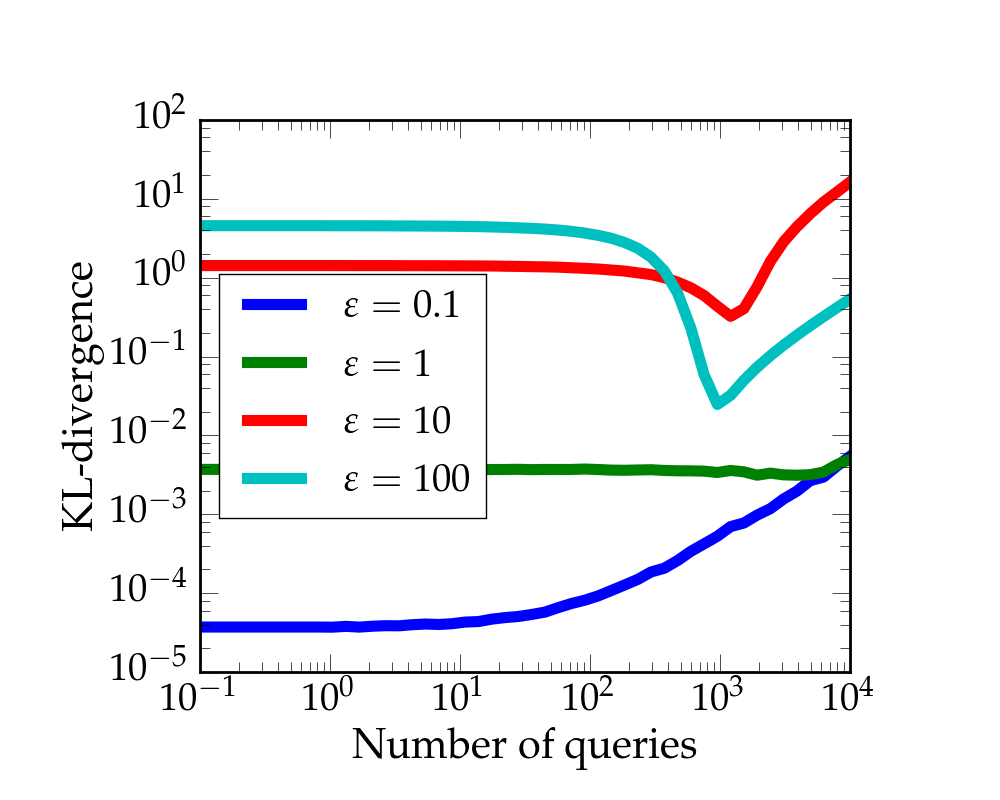
\includegraphics[width=1.2\textwidth]{model1_KL.png}
\caption{The KL divergence of the adversary's approximate probability distribution relative to the true probability distribution of Model 1, as a function of the number of queries to the mechanism as well as the privacy parameter \(\varepsilon\). For the blue line, the probability a given sampled song was \emph{intended} was 10\%; for the green line it was 10\%; for the red line it was 69\%; for the cyan line it was 100\%.}
\end{figure}

Figure~1 demonstrates the opposite result from what we expected. Since a lower \(\varepsilon\) leads to more probability mass on unintended outputs --- more noise --- we expected the adversary to be hindered in his attempts to reconstruct the true probability distribution. Reality is quite the otherwise --- we see that the KL divergence starts out lower for lower \(\varepsilon\). The reason for this is that the Multiplicative Weights algorithm starts by assigning equal probabilities to each output, which is the limit of the true probability distribution as \(\varepsilon \rightarrow 0\). Therefore, for small \(\varepsilon\) a uniform probability distribution accurately approximates the true probability distribution.

A somewhat curious 

\subsection{Model 2}

\section{Conclusions}

\section{Further Work}

There is much further work to be done in this area. A limitation of our Model 1 is that it does not support interactivity, even though it could be easily extended to do so. Further, more methods for quantifying the ease of reconstruction of a content base should be explored, as well as alternative reconstruction strategies for the adversary. A ``Model 3'' might relax the Markovian property of Model 2 so that content-node transition probabilities can depend on the full sequence so far --- this would provide a more general toolkit for content-production.

The biggest challenge the authors faced was defining exactly what could be protected from an adversary. In this paper, we settled with the attempting to protect the probabilities of various outputs, but we are not fully satisfied with this definition. More work should be put into exploring exactly what features of creative works can be protected from reconstruction without significant impacting the enjoyment of the work by authorized users.

%%%%%%%%%%%
\end{document}
